\begin{appendices}
\chapter{Example Darwin Core Archive}\label{appendix:dwc}
\lstinputlisting[caption={EML File},language=XML]{Chap4/listings/dwc_arch/eml.xml}
\lstinputlisting[caption={Metadata File},language=XML]{Chap4/listings/dwc_arch/meta.xml}
\lstinputlisting[caption={Example Set File (set.csv)}]{Chap4/listings/dwc_arch/set.csv}
\lstinputlisting[caption={File Describing Image Locations (images.csv)}]{Chap4/listings/dwc_arch/images.csv}

\chapter{Darwin-SW Occurrence Example}\label{appendix:dsw}
\begin{lstlisting}[language=XML, caption={Darwin-SW Representation of a Living Specimen}]
<?xml version="1.0" encoding="UTF-8"?>
<rdf:RDF xmlns:rdf="http://www.w3.org/1999/02/22-rdf-syntax-ns#"
                 xmlns:rdfs="http://www.w3.org/2000/01/rdf-schema#"
                 xmlns:dcterms="http://purl.org/dc/terms/"
                 xmlns:dwc="http://rs.tdwg.org/dwc/terms/"
                 xmlns:dsw="http://purl.org/dsw/"
                 xmlns:mrtg="http://rs.tdwg.org/mrtg/trunk/RDF/mrtg.n3#"
                 xmlns:xmp="http://ns.adobe.com/xap/1.0/"
                 xmlns:foaf="http://xmlns.com/foaf/0.1/"
                 >

  <rdf:Description rdf:about="http://bioimages.vanderbilt.edu/vanderbilt/12-126">
        <rdf:type rdf:resource="http://purl.org/dsw/IndividualOrganism" />
        <rdf:type rdf:resource="http://purl.org/dsw/LivingSpecimen" />
        <mrtg:metadataLanguage>en</mrtg:metadataLanguage>
        
        <!--Basic information about the individual organism-->
        <dcterms:identifier>http://bioimages.vanderbilt.edu/vanderbilt/12-126</dcterms:identifier>
        <dcterms:description>Field individual of Ginkgo biloba L. with GUID: http://bioimages.vanderbilt.edu/vanderbilt/12-126</dcterms:description>
        <dsw:individualOrganismRemarks>This tree was miraculously spared from destruction in the building of the 21st Ave. crosswalk.</dsw:individualOrganismRemarks>
        
        <!-- Properties that the tree has by virtue of its LivingSpecimen type -->
        <dwc:collectionID rdf:resource="http://biocol.org/urn:lsid:biocol.org:col:35259" />
        <dwc:collectionCode>vanderbilt</dwc:collectionCode>
        <dwc:catalogNumber>12-126</dwc:catalogNumber>
        
        <!-- Relationships of the individual to other resources.  -->
        <foaf:isPrimaryTopicOf rdf:resource="http://bioimages.vanderbilt.edu/vanderbilt/12-126.rdf" />
        <foaf:isPrimaryTopicOf rdf:resource="http://bioimages.vanderbilt.edu/vanderbilt/12-126.htm" />

        
        <!-- Images that are derived from the individual -->
        <foaf:depiction rdf:resource="http://bioimages.vanderbilt.edu/baskauf/10502"/>
        <foaf:depiction rdf:resource="http://bioimages.vanderbilt.edu/baskauf/10557"/>
        <foaf:depiction rdf:resource="http://bioimages.vanderbilt.edu/baskauf/10556"/>
        <foaf:depiction rdf:resource="http://bioimages.vanderbilt.edu/baskauf/10554"/>
        
        <!-- Documented occurrences of the individual -->
        <dsw:hasOccurrence rdf:resource="http://bioimages.vanderbilt.edu/baskauf/10502#occ" />
        <dsw:hasOccurrence rdf:resource="http://bioimages.vanderbilt.edu/baskauf/10557#occ" />
        <dsw:hasOccurrence rdf:resource="http://bioimages.vanderbilt.edu/baskauf/10556#occ" />
        <dsw:hasOccurrence rdf:resource="http://bioimages.vanderbilt.edu/baskauf/10554#occ" />
        
        <!-- Identifications applied to the individual-->
        <dsw:hasIdentification>
          <rdf:Description rdf:about="http://bioimages.vanderbilt.edu/vanderbilt/12-126#2002-04-10baskauf">
                <dcterms:description>Determination of Ginkgo biloba L. sensu Flora of North America (1993) for the individual http://bioimages.vanderbilt.edu/vanderbilt/12-126</dcterms:description>
                <rdf:type rdf:resource="http://rs.tdwg.org/dwc/terms/Identification" />

                <!-- In lieu of stable external identifiers for taxon concepts, Im defining some onsite -->
				<dsw:toTaxon rdf:resource="http://bioimages.vanderbilt.edu/taxonConcepts#183269-fna1993" />
                
				<dwc:identifiedBy>Steven J. Baskauf</dwc:identifiedBy>
                <dsw:idBy rdf:resource="http://bioimages.vanderbilt.edu/contact/baskauf" />
				<dwc:dateIdentified>2002-04-10</dwc:dateIdentified>
                
				<!-- Relationship of the identification to other resources -->
				<dsw:idBasedOn rdf:resource="http://bioimages.vanderbilt.edu/baskauf/10554"/>
          </rdf:Description>
        </dsw:hasIdentification>
  </rdf:Description>

  <!--
		Information about the metadata document itself
  -->
  <rdf:Description rdf:about="http://bioimages.vanderbilt.edu/vanderbilt/12-126.rdf">
        <dcterms:type rdf:resource ="http://xmlns.com/foaf/0.1/Document" />
        <dcterms:identifier>http://bioimages.vanderbilt.edu/vanderbilt/12-126.rdf</dcterms:identifier>
        <dcterms:description>RDF formatted description of the living organism http://bioimages.vanderbilt.edu/vanderbilt/12-126</dcterms:description>
        <dcterms:creator>Bioimages http://bioimages.vanderbilt.edu/</dcterms:creator>
        <foaf:maker rdf:resource="http://biocol.org/urn:lsid:biocol.org:col:35115" />
        <dcterms:language>en</dcterms:language>
        <dcterms:modified>2010-11-08T11:13:49</dcterms:modified>
        <xmp:MetadataDate>2010-11-08T11:13:49</xmp:MetadataDate>
        <dcterms:references rdf:resource="http://bioimages.vanderbilt.edu/vanderbilt/12-126"/>
        <foaf:primaryTopic rdf:resource="http://bioimages.vanderbilt.edu/vanderbilt/12-126"/>
  </rdf:Description>

</rdf:RDF>
\end{lstlisting}

\chapter{K-HAS Ontology}\label{appendix:ontology}
\lstinputlisting[language=XML, caption={K-HAS Ontology Source Code}]{App/listings/align.owl}

\chapter{Example Drools Rules Used in LORIS}\label{appendix:drools}
\lstinputlisting[caption={Example Drools File}]{Chap4/listings/rules.drl}

\chapter{Interview Transcript: Gill Bolongon}\label{appendix:interview}
\lstinputlisting[caption={Sample Intrview Transcript}]{App/listings/Gill.txt}

\chapter{Qualitative Analysis Extract}\label{appendix:interview:extract}
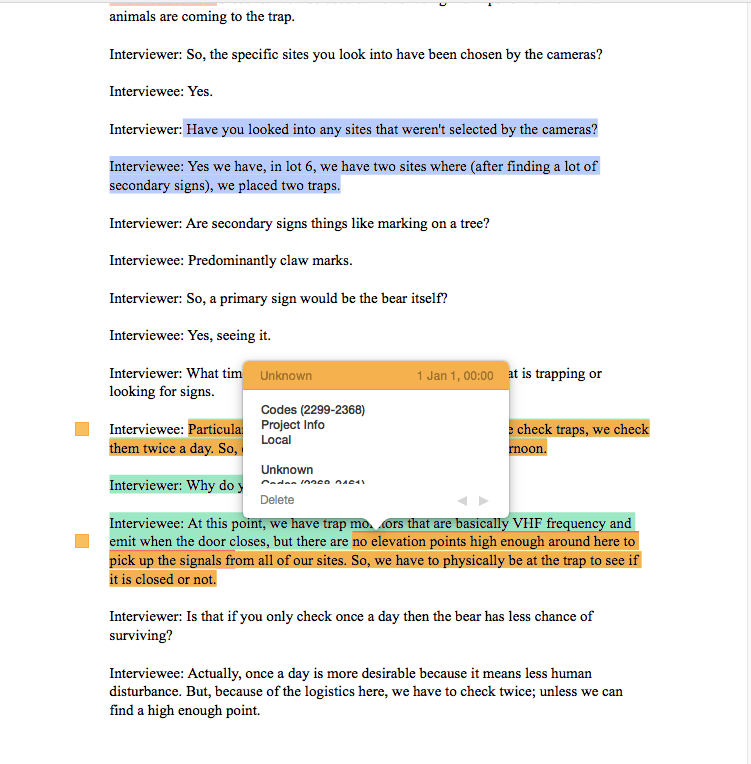
\includegraphics[width=\textwidth]{App/figures/roshan_extract}
\end{appendices}